\section{2021 Вариант 1}

\begin{prob}
Кабина лифта массы $M$ может без трения двигаться в вертикальном направлении в лифтовой шахте. Кабина соединена с потолком шахты системой блоков (см. рис. 1). Груз $m$ может свободно двигаться в вертикальном направлении. Все нити невесомы, нерастяжимы и всегда натянуты (не сминаются). Массой блоков и трением в осях можно пренебречь.
\begin{itemize}
\item[]
\item[(a)] При каких значениях масс $m$ и $M$ кабина лифта может находиться в состоянии покоя?
\item[(б)] Найдите величину силы реакции $N$, действующей на груз со стороны кабины лифта, при $m=M / 2$.
\end{itemize}
\begin{figure}[h!]
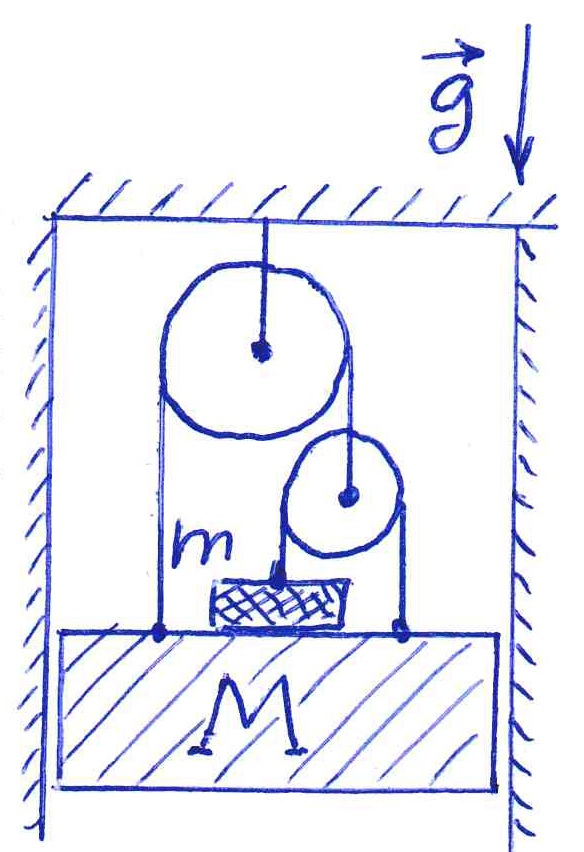
\includegraphics[scale=0.25]{IMG/img_1}
\end{figure}
\end{prob}

\begin{proof}
\begin{itemize}
\item[]
\item[(a)]
    \begin{gather*}
        \ddot{x_1} = \ddot{x_2} = 0\\
        mg = T + N\\
        Mg = 3T - N\\
        \left(M + m\right)g = 4T\Rightarrow
        M = \frac{4T}{g} - m
    \end{gather*}
    Груз не двигается при $\frac{\left(M + m\right)g}{4} < mg$ то есть $M < 3m$
\item[(б)]
    \begin{gather*}
        \frac{M}{2} \ddot{x_1} = \frac{M}{2}g - T - N\\
        M \ddot{x_2} = Mg - 3T + N\\
        \begin{cases}
            \frac{Mx}{2} = \frac{M}{2} g - T - N \qquad \ddot{x_1} = \ddot{x_2} = x\\
            Mx = Mg - 3T + N
        \end{cases}\\
        \Rightarrow
        3N = T\\
        N = \frac{T}{3}
    \end{gather*}
\end{itemize}
\end{proof}
\vskip 0.6in




\begin{prob}
Материальная точка движется вдоль прямой $O x$ в поле потенциальной силы, потенциальная энергия $U(x)$ которой дается выражением:
$$
U(x) =
\begin{cases}
    1-e^{-8 x^2} & x \leq 0 \\
    8 x^2\left(1-x^2\right) & x>0
\end{cases}
$$
\begin{itemize}
\item[]
\item[(a)] Нарисуйте качественный фазовый портрет этой одномерной механической системы.
\item[(б)] Укажите число различных фазовых кривых, отвечающих значениям полной механической энергии $E=0, E=1$ и $E=2$.
\end{itemize}
\end{prob}

\begin{proof}
\begin{itemize}
\item[(a)]
\item[]
    \begin{figure}[h!]
    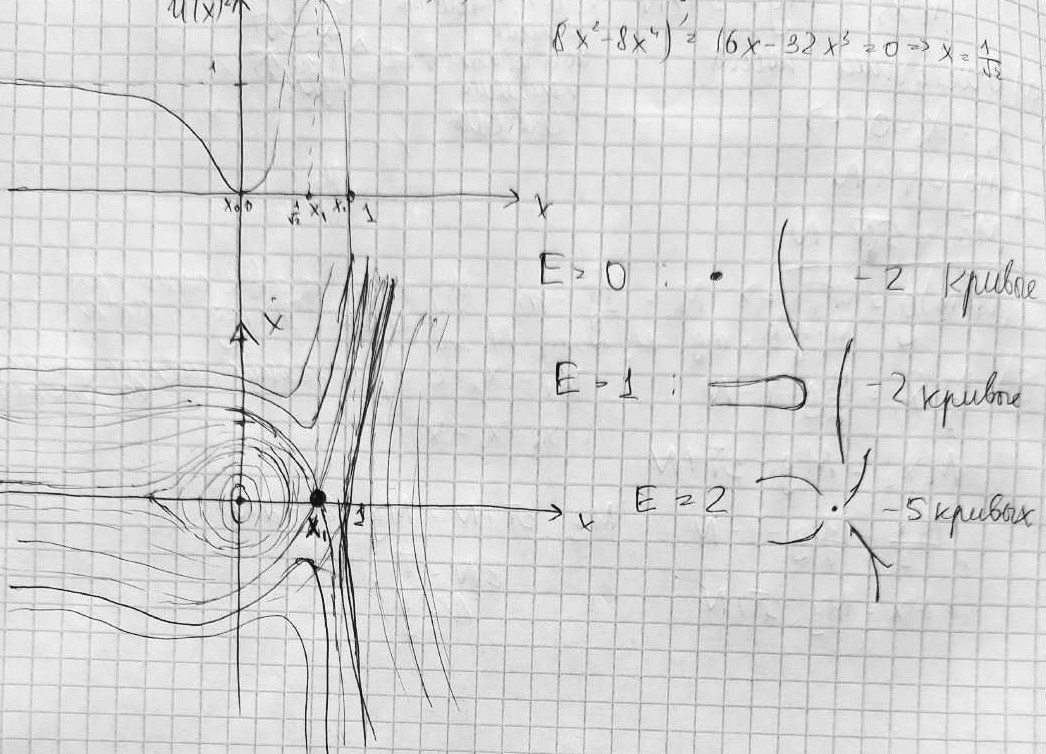
\includegraphics[scale=0.55]{IMG/prb_2v1}
    \end{figure}
\item[(б)]
    \begin{flushleft}
    \begin{tabular}{ c | c c c }
    E & 0 & 1 & 2\\
    Num & 2 & 2 & 5
    \end{tabular}
    \end{flushleft}
\end{itemize}
\end{proof}
\vskip 0.6in




\begin{prob}
Силовое поле $\vec{F}$ задано в декартовых прямоугольных координатах $(x, y, z)$ пространства $\mathbb{R}^3$ следующими выражениями своих компонент:
$$
F_x=2 x y+y, \quad F_y=-2 \alpha y z+x^2+x, \quad F_z=\alpha z-y^2
$$
где $\alpha-$ вещественный числовой параметр.
\begin{itemize}
\item[]
\item[(а)] Найдите работу силы $\vec{F}$ вдоль отрезка кривой, заданной уравнениями
$$
x=y, \quad z=y^2
$$
от начальной точки $\left(0,0,0\right)$ до конечной точки $\left(1,1,1\right)$.
\item[(б)] Определите значение параметра $\alpha$, при котором сила $\vec{F}$ потенциальна, и найдите выражение для соответствующей потенциальной энергии $U(x, y, z)$.
\end{itemize}
\end{prob}

\begin{proof}
\begin{itemize}
\item[]
\item[(a)]
    \begin{gather*}
        d_{\vec{r}} = \left(dt, dt, 2tdt\right)\\
        A = \int\limits_{0}^{1} \left(\left(2xy+y\right)dt + \left(-2\alpha yz + x^2 + x\right)dt + 2t\left(\alpha z - y^2\right)dt\right)\\
        = \int\limits_{0}^{1} \left(2t^2 + t^2 - 2 \alpha t^3 + t^2 + t + 2 t^3 \alpha - 2t^3\right)dt\\
        = \int\limits_{0}^{1} \left(3t^2 + 2t - 2t^3\right)dt
        = t^3 + t^2 - \frac{t^4}{2} \bigg|_{0}^{1}
        = \frac{1}{2}
    \end{gather*}
\item[(б)]
    \begin{gather*}
        \begin{cases}
            \partial_x F_y = \partial_y F_x\\
            \partial_y F_z = \partial_z F_y\\
            \partial_z F_x = \partial_x F_z
        \end{cases}
        \Leftrightarrow
        \begin{cases}
            2x + 1 = 2x + 1\\
            -2y = -2\alpha y\\
            0 = 0
        \end{cases}
        \Leftrightarrow
        \alpha = 1\\
        \partial_x U = -F_x = -2xy - y \Leftrightarrow
        U = -x^2 y - yx + c_1\left(y,z\right)\\
        \partial_y U = -F_y = 2yz - x^2 - x  \Leftrightarrow
        -x^2 - x + c'_{1y} = 2yz - x^2 - x\qquad
        c_1 = y^2 z + c_2\left(z\right)\\
        \partial_z U = -F_z = y^2 - z \Leftrightarrow
        y^2 + c'_2 = y^2 - z\qquad c'_2 = -z\quad c_2 = -\frac{z^2}{2} + c\\
        U\left(x,y,z\right) = -x^2 y - y x + y^2 z - \frac{z^2}{2} + c
    \end{gather*}
\end{itemize}
\end{proof}
\vskip 0.6in




\begin{prob}
Компоненты силы $\vec{F}$ заданы в полярных координатах $(\rho, \phi)$ пространства $\mathbb{R}^2$ следующими выражениями:
$$
F_\rho=\rho f(\phi), \quad F_\phi=g(\rho) \cos ^3 \phi
$$
где $f(\phi)$ и $g(\rho)$ некоторые дифференцируемые функции своих аргументов.
\begin{itemize}
\item[(a)] Определите наиболее общий вид функций $f(\phi)$ и $g(\rho)$, при которых сила $\vec{F}$ потенциальна и не имеет сингулярности в начале координат $\rho=0$.
\item[(б)] Найдите вид соответствующей потенциальной энергии $U(\rho, \phi)$.
\end{itemize}
\end{prob}

\begin{proof}
\begin{itemize}
\item[]
\item[(a)]
    \begin{gather*}
        \partial_{\phi} F_p
        = \partial_{\rho} \left(\rho F_{\phi}\right)\\
        \partial_{\phi} f(\phi)
        = \cos^3 \phi g(\rho) + \partial_{\rho} y \rho \cos^{3} \phi
        = \cos^3 \phi \left(g + \frac{\partial g}{\partial \rho}\rho\right)\\
        \frac{d f}{d \phi} = k \cos^3 \phi\qquad
        \frac{d g}{d \rho} p = k\\
        f(\phi) = k \int \cos^3 \phi d \phi = k \left(\sin \phi - \frac{\sin^3 \phi}{3} + c\right)\\
        g(\rho) \rho = k \int 1 d \rho = kp + c \Rightarrow
        g = k + \frac{c}{p}\\
        F_{\rho} = k \left(\sin \phi - \frac{\sin^3 \phi}{3} + c_1\right) \rho,\qquad
        F_{\phi} = \left(k + \frac{c_2}{p}\right) \cos^3 \phi\qquad
        c_2 = 0
    \end{gather*}
\item[(б)]
    \begin{gather*}
        \nabla = \left(\partial \rho, \frac{1}{\rho} \partial \phi\right)\\
        -\partial_{\rho} U = K \left(\sin \phi - \frac{\sin^3 \phi}{3} + c_1\right)\rho\\
        U = -k \left(\sin \phi - \frac{\sin^3 \phi}{3} + c_1\right) \frac{\rho^2}{2} - c(\phi)\\
        -\frac{1}{\rho} \partial_{\phi} U = -\frac{1}{\rho}\left(\left(-k \cos \phi - \frac{\sin^2 \phi \cos \phi}{3}\right)f^2 + c(\phi)\right)
        = k \cos^3 \phi + \frac{c_2}{\rho} \cos^3 \phi
    \end{gather*}
\end{itemize}
\end{proof}
\newpage




\section{2021 Вариант 2}

\begin{prob}
Кабина лифта массы $M$ может без трения двигаться в вертикальном направлении в лифтовой шахте. Кабина соединена с потолком шахты системой блоков (см. рис. 1). Груз $m$ может свободно двигаться в вертикальном направлении. Все нити невесомы, нерастяжимы и всегда натянуты (не сминаются). Массой блоков и трением в осях можно пренебречь.
\begin{itemize}
\item[(a)] При каких значениях масс $m$ и $M$ кабина лифта может находиться в состоянии покоя?
\item[(б)] Найдите величину силы реакции $N$, действующей на груз со стороны кабины лифта, при $m=M$.
\end{itemize}
\begin{figure}[h!]
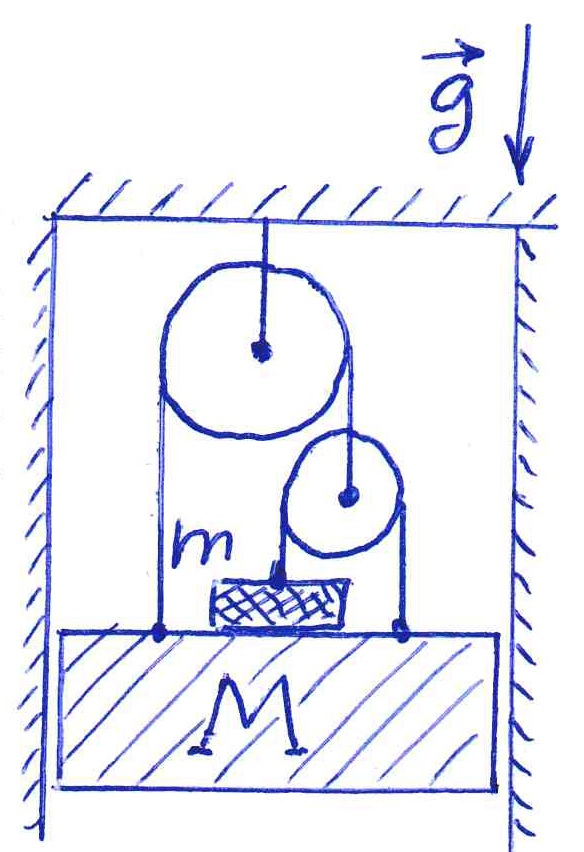
\includegraphics[scale=0.25]{IMG/img_1}
\end{figure}
\end{prob}

\begin{proof}
\begin{itemize}
\item[]
\item[(a)]
    \begin{gather*}
        \ddot{x_1} = \ddot{x_2} = 0\\
        mg = T + N\\
        Mg = 3T - N\\
        \left(M + m\right)g = 4T\Rightarrow
        M = \frac{4T}{g} - m
    \end{gather*}
    Груз не двигается при $\frac{\left(M + m\right)g}{4} < mg$ то есть $M < 3m$
\item[(б)]
    \begin{gather*}
        m = M\qquad \ddot{x_1} = \ddot{x_2}\\
        \begin{cases}
            m\ddot{x_2} = mg - N - T\\
            m\ddot{x_1} = mg + N - 3T
        \end{cases}\\
        -2N + 2T = 0 \Rightarrow N = T 
    \end{gather*}
\end{itemize}
\end{proof}
\vskip 0.6in




\begin{prob}
Материальная точка движется вдоль прямой $O x$ в поле потенциальной силы, потенциальная энергия $U(x)$ которой дается выражением:
$$
U(x) =
\begin{cases}
    e^{-x^2}-1 & x \leq 0 \\
    \frac{1}{3} x^2\left(x-3\right) & x>0
\end{cases}
$$
\begin{itemize}
\item[(a)] Нарисуйте качественный фазовый портрет этой одномерной механической системы.
\item[(б)] Укажите число различных фазовых кривых, отвечающих значениям полной механической энергии $E=-1, E=1/2$ и $E=0$.
\end{itemize}
\end{prob}

\begin{proof}
\begin{itemize}
\item[(a)]
\item[]
    \begin{figure}[h!]
    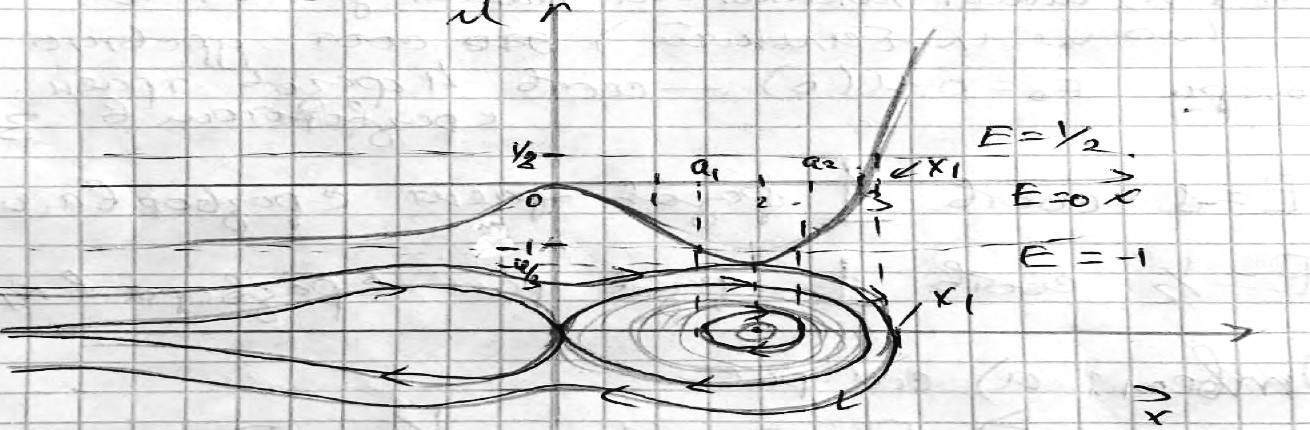
\includegraphics[scale=0.5]{IMG/prb_2v2}
    \end{figure}
\item[(б)]
    \begin{flushleft}
    \begin{tabular}{ c | c c c }
    E & -1 & 1/2 & 0\\
    Num & 1 & 1 & 4
    \end{tabular}
    \end{flushleft}
\end{itemize}
\end{proof}
\vskip 0.6in




\begin{prob}
Силовое поле $\vec{F}$ задано в декартовых прямоугольных координатах $(x, y, z)$ пространства $\mathbb{R}^3$ следующими выражениями своих компонент:
$$
F_x=y z-y^2+\alpha z, \quad F_y=x z-2 \alpha x y, \quad F_z=x y+\alpha x+z
$$
где $\alpha-$ вещественный числовой параметр.
\begin{itemize}
\item[(а)] Найдите работу силы $\vec{F}$ вдоль отрезка кривой, заданной уравнениями
$$
x=y^2, \quad z=y
$$
от начальной точки $\left(0,0,0\right)$ до конечной точки $\left(1,1,1\right)$.
\item[(б)] Определите значение параметра $\alpha$, при котором сила $\vec{F}$ потенциальна, и найдите выражение для соответствующей потенциальной энергии $U(x, y, z)$.
\end{itemize}
\end{prob}

\begin{proof}
\begin{itemize}
\item[]
\item[(a)]
    \begin{gather*}
        d_{\vec{r}} = \left(2tdt, dt, dt\right)\\
        A = \int\limits_{0}^{1} \left(2t\left(y z-y^2+\alpha z\right)dt + \left(x z-2 \alpha x y\right)dt + \left(x y+\alpha x+z\right)dt\right)\\
        = \int\limits_{0}^{1} \left(2t\left(t^2-t^2+\alpha t\right) + \left(t^3-2 \alpha t^3\right) + \left(t^3+\alpha t^2+t\right)\right)dt\\
        = \int\limits_{0}^{1} \left(3 \alpha t^2 + 2\left(1 - \alpha\right)t^3 + t\right)dt
        = \alpha t^3 + \frac{\left(1 - \alpha\right) t^4}{2} + \frac{t^2}{2} \bigg|_{0}^{1}
        = \alpha + \frac{\left(1 - \alpha\right)}{2} + \frac{1}{2}
        = \frac{2 + \alpha}{2}
    \end{gather*}
\item[(б)]
    \begin{gather*}
        \begin{cases}
            \partial_x F_y = \partial_y F_x\\
            \partial_y F_z = \partial_z F_y\\
            \partial_z F_x = \partial_x F_z
        \end{cases}
        \Leftrightarrow
        \begin{cases}
            z - 2 \alpha y = z - 2y\\
            y + \alpha = y + \alpha\\
            x = x
        \end{cases}
        \Leftrightarrow
        \alpha = 1\\
        d U = -\left(\vec{F}, d \vec{r}\right)
        = -\left(yz - y^2 + z\right)dx - \left(xz - 2xy\right)dy - \left(xy + x + z\right)dz
        = -d\left(yzx - y^2 x + zx + \frac{z^2}{2}\right)\\
        U = -xyz + y^2 x - zx - \frac{z^2}{2} + c
    \end{gather*}
\end{itemize}
\end{proof}
\vskip 0.6in




\begin{prob}
Компоненты силы $\vec{F}$ заданы в полярных координатах $(\rho, \phi)$ пространства $\mathbb{R}^2$ следующими выражениями:
$$
F_\rho=\rho(\rho+1) f(\phi), \quad F_\phi=g(\rho) \cos \phi \sin ^3 \phi
$$
где $f(\phi)$ и $g(\rho)$ некоторые дифференцируемые функции своих аргументов.
\begin{itemize}
\item[]
\item[(a)] Определите наиболее общий вид функций $f(\phi)$ и $g(\rho)$, при которых сила $\vec{F}$ потенциальна и не имеет сингулярности в начале координат $\rho=0$.
\item[(б)] Найдите вид соответствующей потенциальной энергии $U(\rho, \phi)$.
\end{itemize}
\end{prob}

\begin{proof}
\begin{itemize}
\item[]
\item[(a)]
    \begin{gather*}
        \rho \left(\rho + 1\right) f'(\phi)
        = \partial_{\phi} F_p
        = \partial_{\rho} \left(\rho F_{\phi}\right)
        = \cos \phi \sin^3 \phi \left(g(\rho) + \rho g' (\rho)\right)\\
        f'(\phi) = A \cos \phi \sin^3 \phi\qquad
        A \cdot B = 1\\
        \rho \left(\rho + 1\right) = B\left(g(\rho) + \rho g'(\rho)\right)\\
        f(\phi) = A \left(\frac{\sin^4 \phi}{4} + c_1\right)\\
        g(\rho) = \frac{c_2}{\rho} + \frac{\rho^2}{3B} + \frac{\rho}{2B}\\
        F_{\rho} = A \rho \left(\rho + 1\right) \left(\frac{\sin^4 \phi}{4} + c_1\right)\\
        F_{\phi} = \left(\frac{c_2}{\rho} + \frac{\rho^2 A}{3 \rho} + \frac{\rho A}{2}\right) \cos \phi \sin^3 \phi
        = A \rho \left(\frac{\rho}{3} + \frac{1}{2}\right)\cos \phi \sin^3 \phi
    \end{gather*}
\item[(б)]
    \begin{gather*}
        -\partial_{\rho} U
        = F_{\rho}
        = A \rho \left(\rho + 1\right) \left(\frac{\sin^4 \phi}{4} + c_1\right)\\
        -U = A\left(\frac{\rho^3}{3} + \frac{\rho^2}{2}\right)\left(\frac{\sin^4 \phi}{4} + c_1\right) + f(\phi)\\
        A\left(\frac{\rho^3}{3} + \frac{\rho^2}{2}\right)\sin^3 \phi \cos \phi + f'(\phi)
        = -\partial_{\phi} U
        = \rho F_{\phi}
        = A \rho^2 \left(\frac{\rho}{3} + \frac{1}{2}\right) \cos \phi \sin^3 \phi\qquad
        f'(\phi) = 0\\
        U = -A \rho^2 \left(\frac{\rho}{3} + \frac{1}{2}\right)\left(\frac{\sin^4 \phi}{4} + c_1\right) + c_2
    \end{gather*}
\end{itemize}
\end{proof}
\newpage



\section{2022 (оба варианта)}

\begin{prob}
Тележка массы $M_1$ может без трения двигаться по прямой по поверхности горизонтального стола. На тележке шарнирно закреплен жесткий невесомый стержень длины $2 l$, который может свободно вращаться в вертикальной плоскости, параллельной линии движения тележки. Шарнирное крепление расположено в геометрическом центре стержня. На концах стержня закреплеmы одишаковые точечные массы $m$. Невесомая нерастяжимая нить, перекинутая через невесомый блок, соединяет тележку с грузом $M_2$, который двигается вдоль вертикальной прямой. Система находится в однородном постоянном поле тяжести $\vec{g}$, направленном вертикально вниз (см. рисунок).
\begin{itemize}
\item[]
\item[(a)] Определите число степеней свободы системы.
\item[(6)] Выбрав подходящие обобщенные координаты, составьте Лагранжиан системы.
\item[(в)] Выпишите формулы для всех сохраняющихся величин (интегралов движения), которые имеются в данной системе.
\end{itemize}
\begin{figure}[h!]
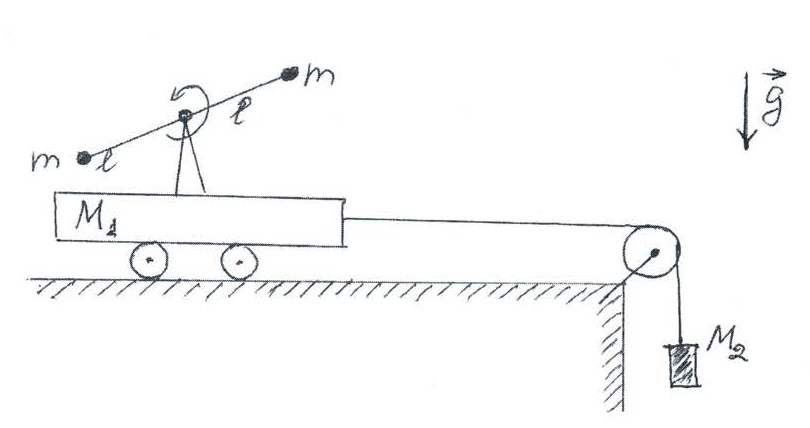
\includegraphics[scale=0.55]{IMG/img_2}
\end{figure}
\end{prob}

\begin{proof}
\begin{itemize}
\item[]
\item[(a)] Заметим что система задается 2 координатами - углом стержня $\phi$ и положением тележки по оси $O x$ (или груза по оси $O y$, в силу нерастяжимости нити эти два параметра эквивалентны).
\item[(б), (в)] 
    \begin{gather*}
        \begin{cases}
            T = M_2 g\\
            N = 2 m g\\
            M_1 g = N_1 + N_2\\
            N_1 = N_2
        \end{cases}\\
    \end{gather*}
\end{itemize}
\end{proof}
\vskip 0.6in




\section{2023 (2 Вариант)}

\begin{prob}
Один конец жесткого невесомого стержня длины $R$ закреплен так, что он может свободно врашаться вокруг него в вертикальной плоскости. На другом его конце шарнирно закреплен второй жесткий невесомый стержень длины $2l$. Шарнирное крепление расположено посередине второго стержны, и он может вращаться вокрут крепления в той же вертикальной плоскости. На кощцах вгорого стержня закреплены одинаковые точечные массы $m$. Система находигся в однородном постоянном поде тяжести с ускорением свободного надения $\vec{g}$, направленным вертикально вниз (см. рисунок). Трение отсутствует.
\begin{itemize}
\item[]
\item[(a)] Определите число степеней свободы системы.
\item[(6)] Выбрав подходящие обобщенные координаты, составьте Лагранжиан системы.
\item[(в)] Выпишите выражения для всех законов сохранения (интегралов движения), которые имеются в данной системе.
\end{itemize}
\begin{figure}[h!]
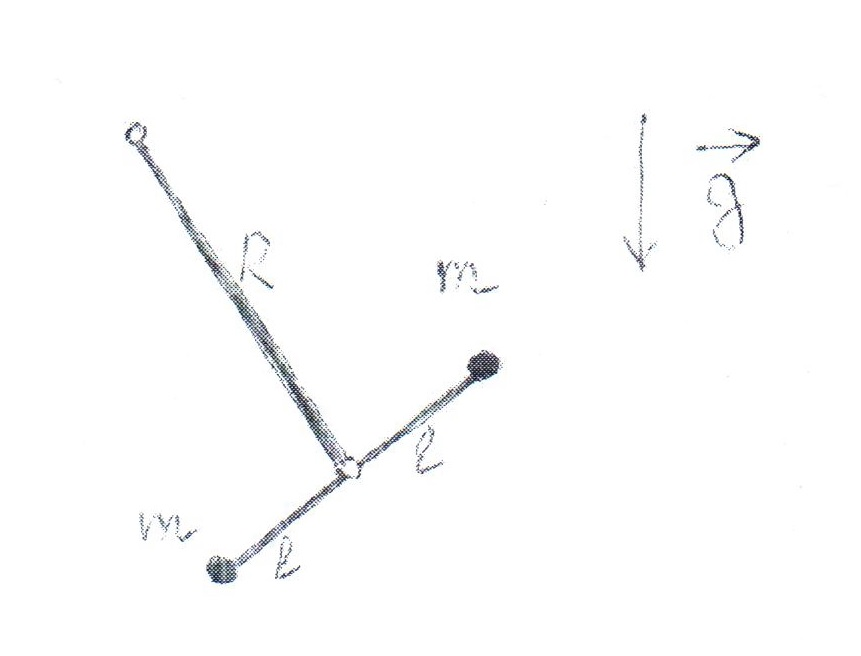
\includegraphics[scale=0.55]{IMG/img_3}
\end{figure}
\end{prob}

\begin{proof}
\begin{itemize}
\item[]
\item[(a)] Система полностью задается 2 углами $\phi$ (один из стержней с $O y$), $\theta$ (угол между стержнями)
\item[(б)]
    $c$ - центр масс 
    \begin{gather*}
        T = T_{c} + T_{o}\\
        T_{c} = \frac{m}{2} R \dot{\phi}^2\\
        T_{o} = 2 \cdot \frac{m}{2} l \dot{\theta}^2\\
        T = m (\frac{1}{2} R \dot{\phi}^2 + l \dot{\theta}^2)
        = \frac{m}{2} (R \dot{\phi}^2 + 2 l \dot{\theta}^2)\\
        U = -mg y_1 - mg y_2
        = -mg(R \cos \phi - h) - mg(R \cos \phi + h)
        = -2mgR \cos \phi\\
        L = T - U = \frac{m}{2}(R \dot{\phi}^2 - 2 l \dot{\theta}^2) + 2mgR \cos \phi
    \end{gather*}
\item[(в)]
    ЗСЭ т.к. $\frac{\partial L}{\partial t} = 0$ 
    \begin{gather*}
            T - U = \text{const} \Leftrightarrow
            \frac{m}{2}(R \dot{\phi}^2 - 2 l \dot{\theta}^2) + 2mgR \cos \phi = \text{const}
    \end{gather*}
    ЗС обобщенного импульса для координаты $\theta$
    \begin{gather*}
        \frac{d}{dt} \frac{\partial L}{\partial \dot{\theta}}
        = \frac{\partial L}{\partial \theta}
        = 0 \Rightarrow
        \frac{\partial L}{\partial \dot{\theta}}
        = 2ml \dot{\theta}
        = I = \text{const}
    \end{gather*}
\end{itemize}
\end{proof}